%\newpage
%\section{Заполнение шаблона}
%\begin{itemize}
	%\item Изменить \textbf{config.tex}: имя студента, название предмета и пр. %параметры указаны именно там
	%\item Заполнить \textbf{content.tex} - файл, который будет содержать весь %текст отчёта, от вступления до заключения.
	%\item Добавить используемую литературу (если есть) в \textbf{refs.bib}. Для %удобного поиска источников можно воспользоваться Google Books. Использованные %источники можно указывать с помощью команды \textbf{\\cite\{name\_of\_ref\}}
%\end{itemize}
%Далее представлены различные примеры.

\section{Цель работы}\label{sec:purpose}


Ознакомление с методом ориентации кристаллов путем наблюдения фигур астеризма.
Изучение кристаллографии кубических кристаллов.


\section{Задачи, решаемые в лабораторной работе}\label{sec:tasks}
\begin{enumerate}
	\item{Научиться определять в градусной мере ориентацию кристаллов путем фиксации рефлексов от поверхности.
	Научиться объяснять фигуры астеризма. Ознакомиться с кристаллографией кубических кристаллов.}
	\item Научиться наблюдать фигуры оптического астеризма.
	\item Получить базовые знания по применению сетки Вульфа.
	\item Определить, какую роль играет шлифовка отражающей/преломляющей поверхности образца.
\end{enumerate}

\section{Объект исследования}\label{sec:object}

Объектом исследования в данной работе  являются кристаллы флюорита.
%\section{Теоретическая информация}\label{sec:теоретическая-информация}

%Было использовано методическое указание по выполнению лабораторного практикума по основам фотоники.
%Исследование кинетических свойств фотохромных стекол~\cite{conlan1983massive}.

%\section{Рабочие формулы и исходные данные}\label{sec:initial_data}

%\begin{equation}
%a= \begin{cases}
% 3x + 5y + z, \mbox{если хорошо} \\
% 7x - 2y + 4z, \mbox{если плохо}\\
% -6x + 3y + 2z, \mbox{если совсем плохо}
%\end{cases}
%\label{eq:F10}
%\end{equation}

%\begin{equation}
%\tau{_{rad}^{-1}} = 8 \cdot \pi \cdot c
%					\cdot n^2 \cdot \tilde{\nu}^2 \cdot \frac{8}{7}
%					\cdot \int \sigma_{abs}(\nu)d\nu
%\label{eq:F1}
%\end{equation}
%где $c$ – скорость света, $n$ – показатель преломления стекла,
%$\tilde{\nu}$ – средняя частота полосы, $\int \sigma_{abs}(\nu)d\nu$
%– интегральное сечение поглощение основного
%резонансного перехода
%${}^4$$I_{15/2}\rightarrow{}^4$$I_{13/2}$
%
%%\rightarrow\sideset{^4}{_{13/2}}I
%\begin{equation}
%q = (\tau_{exp}/\tau_{rad}) \cdot 100\%,
%\label{eq:F2}
%\end{equation}
%где $\tau_{exp}$ – экспериментально определенное время
%жизни люминесценции перехода
%${}^4$$I_{15/2}\rightarrow{}^4$$I_{13/2}$,
%$\tau_{rad}$ – радиационное время жизни люминесценции перехода
%${}^4$$I_{15/2}\rightarrow{}^4$$I_{13/2}$.

\section{Оборудования и принадлежности}\label{sec:stuff}
\subsection{Схема установки}\label{subsec:schemes}
\begin{figure}[H]
        \centering
        \includegraphics[width=0.7\columnwidth]{figures/Scheme}%[width=]
        \caption{Схема экспериментальной установки для измерения ориентации образцов малого размера. 1 - столик, 2 - экран-диафрагма, 3 - экран №2}
		\label{fig:Scheme}
\end{figure}

\section{Результаты эксперимента}\label{sec:results}

Произведя настройку прибора, представленного на рисунке \ref{fig:Scheme},
с помощью Перемещения исследуемого образца под падающим пучком света с экрана №1, было зафиксировано два значения:
угол отклонения  кристаллографической оси [111], и направления, вдоль которого эта ось наклонена в базисе.
Полученные данные записаны в таблицу \ref{tab:base}.

\begin{table}[H]
    \centering
	\begin{threeparttable}% выравнивание подписи по границам таблицы
    % \captionsetup{justification=raggedright} % выравнивание подписи по-центру
    \caption{Координаты рефлексов}\label{tab:base}
    \begin{tabular}{|c|c|c|}
        \hline
		$\delta$x, мм   & $\phi$, \degree & $\rho$, \degree \\ \hline
		0  & 325 & 1   \\ \hline
		1  & 315 & 1   \\ \hline
		2  & 310 & 1,5 \\ \hline
		3  & 310 & 1,5 \\ \hline
		4  & 310 & 1,5 \\ \hline
		5  & 310 & 1,5 \\ \hline
		6  & 285 & 2,5 \\ \hline
		7  & 290 & 2,5 \\ \hline
		8  & 290 & 2,5 \\ \hline
		9  & 290 & 2,5 \\ \hline
		10 & 290 & 2,5 \\ \hline
		11 & 290 & 2,5 \\ \hline
		12 & 290 & 2,5 \\ \hline
		13 & 300 & 2   \\ \hline
		14 & 300 & 2   \\ \hline
		15 & 300 & 2   \\ \hline
		16 & 295 & 2   \\ \hline
		17 & 295 & 2   \\ \hline
		18 & 290 & 2,5 \\ \hline
		19 & 290 & 2,5 \\ \hline
		20 & 285 & 2,5 \\ \hline
		21 & 55  & 0,5 \\ \hline
		22 & 55  & 0,5 \\ \hline
    \end{tabular}
	\end{threeparttable}
\end{table}

Получены графические зависимости $\rho(x)$ (Рисунок - \ref{fig:rhox})  и $\phi(x)$ (Рисунок - \ref{fig:phix}).

\begin{figure}[H]
        \centering
        \includegraphics[width=0.7\columnwidth]{figures/rhox}%[width=]
        \caption{Зависимость $\rho(x)$}
		\label{fig:rhox}
\end{figure}

\begin{figure}[H]
        \centering
        \includegraphics[width=0.7\columnwidth]{figures/phix}%[width=]
        \caption{Зависимость $\phi(x)$}
		\label{fig:phix}
\end{figure}

Построены полученные значения на сетке Вульфа (Рисунок - \ref{fig:wulffnet}).
Для большей наглядности умножили $\rho$ на коэффициент $k$ = 10.
В дальнейших расчетах это было учтено.

\begin{figure}[H]
        \centering
        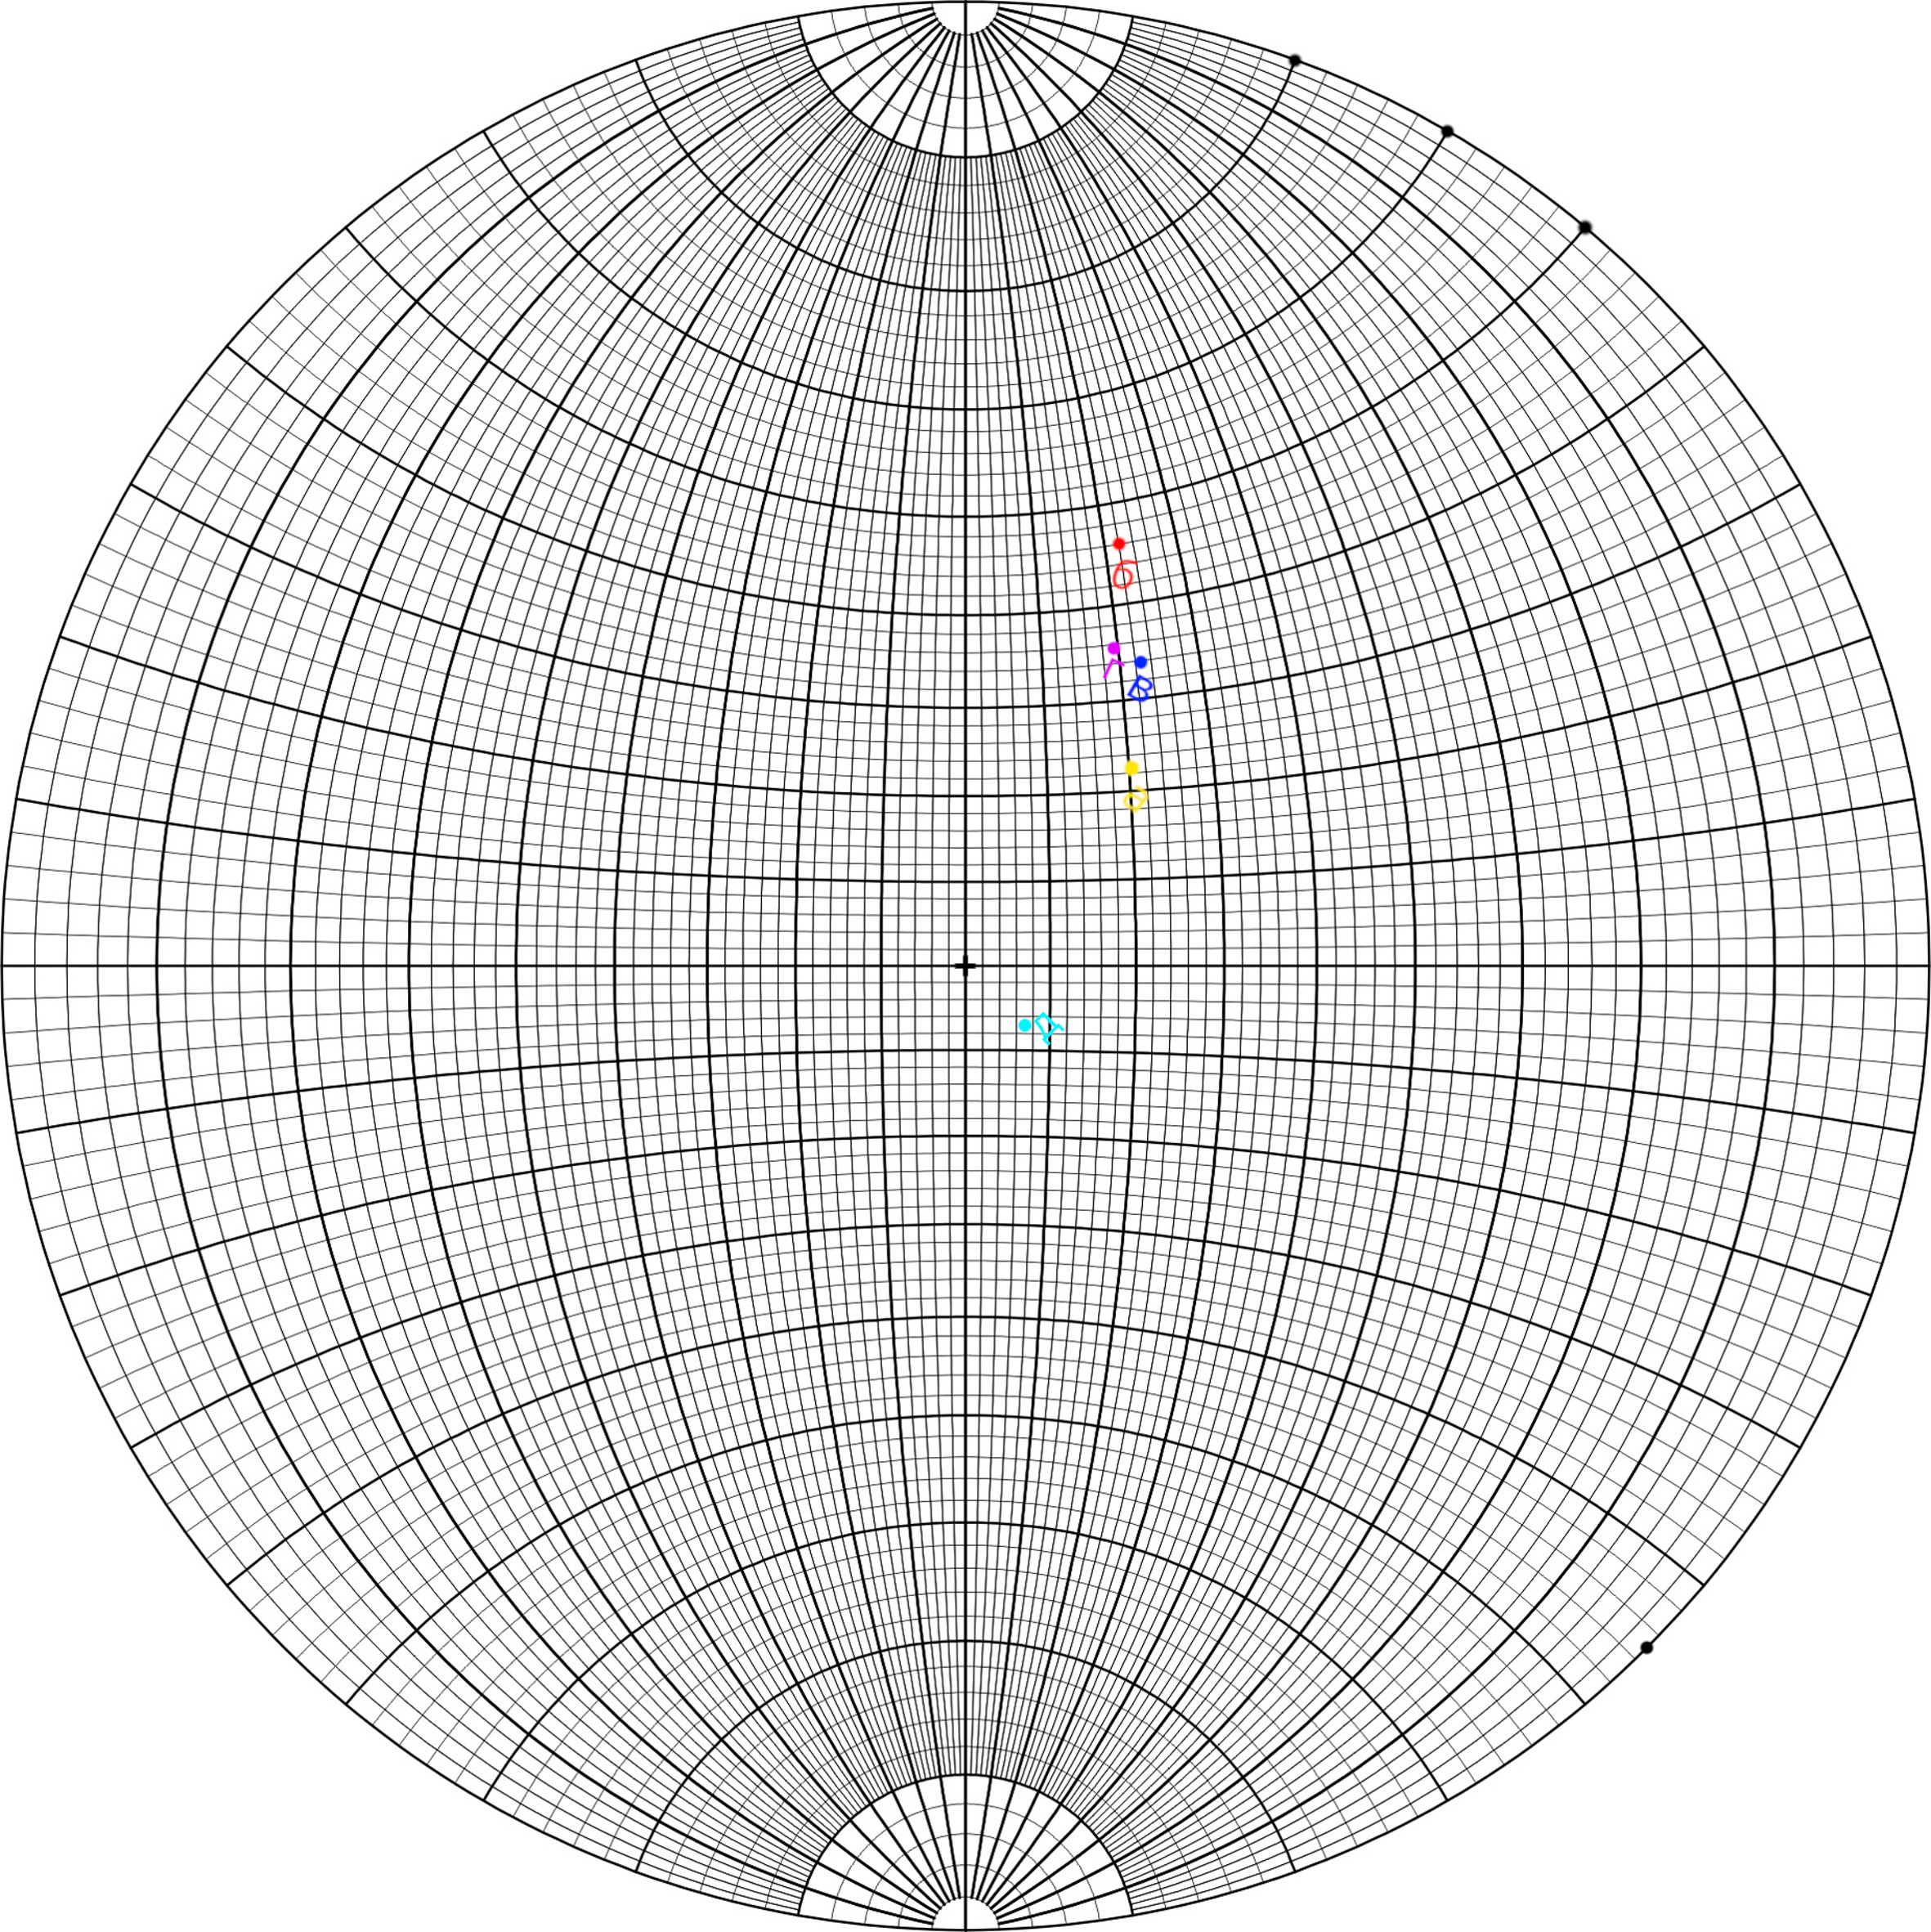
\includegraphics[width=0.7\columnwidth]{figures/wulffnet}%[width=]
        \caption{Стереографические проекции направлений [111], заданных сферическими координатами $\phi$ и $\rho$, сетка Вульфа}
		\label{fig:wulffnet}
\end{figure}

С помощью сетки Вульфа было по меридиональной дуге были измерены градусы между проекциями,
соответствующими направлениям [111] для каждой пары блоков (Таблица - \ref{tab:angel}).

\begin{table}[H]
    \centering
	\begin{threeparttable}% выравнивание подписи по границам таблицы
    % \captionsetup{justification=raggedright} % выравнивание подписи по-центру
    \caption{Угол между направлениями проекций [111]}\label{tab:angel}
    \begin{tabular}{|c|c|}
        \hline
		Проекции & $\phi$, \degree  \\ \hline
		А и Б & 2,3 \\ \hline
		А и В & 1,2 \\ \hline
		А и Г & 1,3 \\ \hline
		А и Д & 3   \\ \hline
		Б и В & 1   \\ \hline
		Б и Г & 1   \\ \hline
		Б и Д & 5,5 \\ \hline
		В и Г & 0,4 \\ \hline
		В и Д & 4,2 \\ \hline
		Г и Д & 4,3 \\ \hline
    \end{tabular}
	\end{threeparttable}
\end{table}

\section{Выводы и анализы результатов}\label{sec:conclution}

В ходе лабораторной работы были проведены измерения угла отклонения кристаллографической оси [111], а также направление отраженных лучей на экране 1
от поверхности кристалла флюорита.
Исследуя поверхность флюорита, были найдены и занесены на графики 3 кристаллографических блоков.
Были найдены углы между различными направлениями проекций [111].

